\section{Authorization}

\subsection{Introduction to Authorization}

\begin{definition}{Authorization}\\
Authorization is the process of determining whether an authenticated entity is permitted to perform a requested action:
\begin{itemize}
    \item Follows successful authentication
    \item Controls access to resources and operations
    \item Implements security policies
    \item Enforces principle of least privilege
\end{itemize}
\end{definition}

\begin{concept}{Fundamental Building Blocks}\\
Authorization systems consist of three core components:
\begin{itemize}
    \item \textbf{Access Control Model} - Conceptual framework defining how access decisions are made
    \item \textbf{Security Policy} - Rules defining who can access what resources
    \item \textbf{Security Mechanism} - Technical implementation enforcing the security policy
\end{itemize}
\end{concept}

\begin{theorem}{Security Policy Drivers}\\
Security policies are influenced by multiple factors:
\begin{itemize}
    \item \textbf{Business Drivers} - Efficiency, usability, operational requirements
    \item \textbf{Security Drivers} - Risk management, threat mitigation, data protection
    \item \textbf{Regulatory Drivers} - Legal compliance, industry standards
\end{itemize}
\end{theorem}

\subsection{Access Control Models}

\begin{concept}{Major Access Control Models}\\
Three primary access control models dominate modern systems:
\begin{itemize}
    \item \textbf{Discretionary Access Control (DAC)} - Access decisions made by resource owners
    \item \textbf{Mandatory Access Control (MAC)} - Access decisions enforced by system policy
    \item \textbf{Role-Based Access Control (RBAC)} - Access based on user roles within an organization
\end{itemize}
Additional models include:
\begin{itemize}
    \item \textbf{Attribute-Based Access Control (ABAC)} - Access based on attributes of users, resources, and environment
    \item \textbf{Rule-Based Access Control} - Access based on predefined rules
    \item \textbf{Relationship-Based Access Control (ReBAC)} - Access based on relationships between entities
\end{itemize}
\end{concept}

\subsection{Discretionary Access Control (DAC)}

\begin{definition}{Discretionary Access Control}\\
DAC is an access control model where the resource owner controls access rights:
\begin{itemize}
    \item Resource owners determine who can access their resources
    \item Owners can delegate access control to others
    \item Access rights can be transferred between users
    \item Most common model in general-purpose operating systems
\end{itemize}
\end{definition}

\begin{concept}{DAC Implementation Methods}\\
DAC is commonly implemented through two main mechanisms:
\begin{itemize}
    \item \textbf{Access Control Lists (ACLs)}:
    \begin{itemize}
        \item Lists of permissions attached to objects
        \item Each entry specifies subject and allowed operations
        \item Efficiently answers "who can access this object?"
    \end{itemize}
    \item \textbf{Capabilities}:
    \begin{itemize}
        \item Unforgeable tokens owned by subjects
        \item Each token grants specific access rights
        \item Efficiently answers "what can this subject access?"
    \end{itemize}
\end{itemize}
\end{concept}

\begin{theorem}{DAC Advantages and Disadvantages}\\
DAC offers certain benefits and limitations:
\begin{itemize}
    \item \textbf{Advantages}:
    \begin{itemize}
        \item Flexible and intuitive for users
        \item Simple to understand and administer
        \item Enables fine-grained access control
    \end{itemize}
    \item \textbf{Disadvantages}:
    \begin{itemize}
        \item Vulnerable to Trojan horse attacks
        \item Cannot enforce system-wide security policies
        \item May lead to uncontrolled information flow
        \item Prone to privilege creep over time
    \end{itemize}
\end{itemize}
\end{theorem}

\subsection{UNIX/Linux File Permissions}

\begin{definition}{Standard UNIX Permissions}\\
UNIX-style file permissions implement a simple form of DAC:
\begin{itemize}
    \item Each file/directory has an owner and group
    \item Permissions divided into three categories:
    \begin{itemize}
        \item Owner (user) permissions
        \item Group permissions
        \item Others (world) permissions
    \end{itemize}
    \item Each category can have read (r), write (w), and execute (x) permissions
    \item Represented as 9 bits, often shown in octal notation (e.g., 755)
\end{itemize}
\end{definition}

\begin{concept}{UNIX Permission Interpretation}\\
Permission bits have different meanings for files and directories:
\begin{itemize}
    \item \textbf{For Files}:
    \begin{itemize}
        \item Read (r) - View file contents
        \item Write (w) - Modify file contents
        \item Execute (x) - Run file as a program
    \end{itemize}
    \item \textbf{For Directories}:
    \begin{itemize}
        \item Read (r) - List directory contents
        \item Write (w) - Create, delete, or rename files within directory
        \item Execute (x) - Access files and subdirectories (traverse)
    \end{itemize}
\end{itemize}
\end{concept}

\begin{code}{Managing UNIX Permissions}\\
\begin{lstlisting}[language=bash, style=basesmol]
# Display file permissions
ls -l myfile.txt
# -rw-r--r-- 1 alice users 2048 Apr 15 14:22 myfile.txt
#  ^ ^ ^  ^
#  | | |  |
#  | | |  +-- Others: read only
#  | | +---- Group: read only
#  | +------ Owner: read and write
#  +-------- File type (regular file)

# Change permissions using symbolic notation
chmod u+x myfile.txt     # Add execute permission for owner
chmod g+w myfile.txt     # Add write permission for group
chmod o-r myfile.txt     # Remove read permission for others
chmod a+x myfile.txt     # Add execute permission for all categories

# Change permissions using octal notation
chmod 755 myfile.txt     # rwxr-xr-x (Owner: rwx, Group: r-x, Others: r-x)
chmod 644 myfile.txt     # rw-r--r-- (Owner: rw-, Group: r--, Others: r--)
chmod 700 myfile.txt     # rwx------ (Owner: rwx, Group: ---, Others: ---)

# Change owner and group
chown alice:users myfile.txt
\end{lstlisting}
\end{code}

\begin{concept}{Special Permission Bits}\\
UNIX systems have additional permission bits for special purposes:
\begin{itemize}
    \item \textbf{Setuid bit (4000)} - When set on executable files, the program runs with the permissions of the file owner
    \item \textbf{Setgid bit (2000)}:
    \begin{itemize}
        \item On executable files: Program runs with the permissions of the file's group
        \item On directories: New files inherit the directory's group
    \end{itemize}
    \item \textbf{Sticky bit (1000)} - On directories, files can only be deleted or renamed by their owner (commonly used on /tmp)
\end{itemize}
\end{concept}

\begin{KR}{Effective UNIX Permission Management}\\
\paragraph{File Ownership}
\begin{itemize}
    \item Assign appropriate owner and group to files
    \item Create groups based on access requirements
    \item Use chown and chgrp to modify ownership
\end{itemize}

\paragraph{Permission Assignment}
\begin{itemize}
    \item Follow principle of least privilege
    \item For directories, consider child file implications
    \item Remember execute permission is needed to traverse directories
    \item Use special bits cautiously
\end{itemize}

\paragraph{Default Permissions}
\begin{itemize}
    \item Configure umask to set default permissions
    \item Common umask values:
    \begin{itemize}
        \item 022 - Files: 644, Directories: 755
        \item 027 - Files: 640, Directories: 750
    \end{itemize}
\end{itemize}

\paragraph{Permission Verification}
\begin{itemize}
    \item Regularly audit permissions
    \item Test access with different user accounts
    \item Check effective permissions with access control lists
\end{itemize}
\end{KR}

\subsection{Access Control Lists (ACLs)}

\begin{definition}{POSIX ACLs}\\
POSIX Access Control Lists extend standard UNIX permissions:
\begin{itemize}
    \item Allow specifying permissions for multiple users and groups
    \item Maintain backward compatibility with standard permissions
    \item Include:
    \begin{itemize}
        \item Minimal ACLs - Equivalent to standard permissions
        \item Extended ACLs - Additional users/groups with specific permissions
    \end{itemize}
\end{itemize}
\end{definition}

\begin{concept}{ACL Components}\\
POSIX ACLs consist of several entry types:
\begin{itemize}
    \item \textbf{Owner entry} - Permissions for the file owner (user::rwx)
    \item \textbf{Named user entries} - Permissions for specific users (user:alice:rwx)
    \item \textbf{Group owner entry} - Permissions for the file's group (group::rwx)
    \item \textbf{Named group entries} - Permissions for specific groups (group:developers:rwx)
    \item \textbf{Other entry} - Permissions for everyone else (other::rwx)
    \item \textbf{Mask entry} - Maximum permissions for named users/groups and group owner
\end{itemize}
\end{concept}

\begin{code}{Managing POSIX ACLs}\\
\begin{lstlisting}[language=bash, style=basesmol]
# Display ACLs
getfacl myfile.txt
# file: myfile.txt
# owner: alice
# group: users
# user::rw-
# group::r--
# other::r--

# Add an ACL entry for user bob with read and write permissions
setfacl -m user:bob:rw- myfile.txt

# Add an ACL entry for group developers with read permissions
setfacl -m group:developers:r-- myfile.txt

# View the updated ACLs
getfacl myfile.txt
# file: myfile.txt
# owner: alice
# group: users
# user::rw-
# user:bob:rw-
# group::r--
# group:developers:r--
# mask::rw-
# other::r--

# Remove an ACL entry
setfacl -x user:bob myfile.txt

# Remove all ACLs and revert to standard permissions
setfacl -b myfile.txt
\end{lstlisting}
\end{code}

\begin{example}
A university department sets up a shared project directory for collaboration between faculty and students. They need different permission levels for different groups. They create the directory with standard permissions for the owner (rwx), but then use ACLs to provide tailored access:

\begin{lstlisting}[style=basesmol]
# Create project directory
mkdir /projects/physics101
chmod 700 /projects/physics101

# Set ACLs
# Faculty get full access
setfacl -m group:faculty:rwx /projects/physics101
# Teaching assistants get read and execute
setfacl -m group:tas:r-x /projects/physics101
# Students get read-only
setfacl -m group:students:r-- /projects/physics101
# Department staff gets full access
setfacl -m group:staff:rwx /projects/physics101

# Create subdirectory for submissions with different permissions
mkdir /projects/physics101/submissions
# Students can write to submissions directory
setfacl -m group:students:r-x /projects/physics101/submissions
# Default ACL for new files in submissions directory
setfacl -d -m group:faculty:rwx /projects/physics101/submissions
setfacl -d -m group:tas:r-x /projects/physics101/submissions
setfacl -d -m group:students:r-- /projects/physics101/submissions
\end{lstlisting}

This setup allows faculty to manage all content, TAs to access but not modify most content, and students to read course materials while being able to navigate to the submissions directory where they can add their assignments.
\end{example}

\subsection{Mandatory Access Control (MAC)}

\begin{definition}{Mandatory Access Control}\\
MAC is an access control model where a system-wide policy determines access rights:
\begin{itemize}
    \item Access decisions enforced by the system, not resource owners
    \item Based on security labels assigned to subjects and objects
    \item Security policy defined by system administrators
    \item Users cannot override or modify access controls
\end{itemize}
\end{definition}

\begin{concept}{MAC Implementations}\\
Modern operating systems implement various forms of MAC:
\begin{itemize}
    \item \textbf{SELinux (Security-Enhanced Linux)}:
    \begin{itemize}
        \item Developed by NSA
        \item Label-based access control
        \item Fine-grained policy control
        \item Used in Red Hat/Fedora distributions
    \end{itemize}
    \item \textbf{AppArmor}:
    \begin{itemize}
        \item Path-based access control
        \item Simpler configuration than SELinux
        \item Used in Ubuntu/SUSE distributions
    \end{itemize}
    \item \textbf{Windows Mandatory Integrity Control}:
    \begin{itemize}
        \item Introduced in Windows Vista
        \item Based on integrity levels (Low, Medium, High, System)
        \item Prevents lower integrity processes from modifying higher integrity resources
    \end{itemize}
\end{itemize}
\end{concept}

\begin{theorem}{MAC vs. DAC Comparison}\\
MAC and DAC differ in several key aspects:
\begin{itemize}
    \item \textbf{Control}:
    \begin{itemize}
        \item DAC - Resource owners control access
        \item MAC - System policy controls access
    \end{itemize}
    \item \textbf{Policy Management}:
    \begin{itemize}
        \item DAC - Distributed management
        \item MAC - Centralized management
    \end{itemize}
    \item \textbf{Security Assurance}:
    \begin{itemize}
        \item DAC - Lower, vulnerable to user errors
        \item MAC - Higher, enforces system-wide policy
    \end{itemize}
    \item \textbf{Complexity}:
    \begin{itemize}
        \item DAC - Simpler to implement and understand
        \item MAC - More complex, requires specialized knowledge
    \end{itemize}
\end{itemize}
\end{theorem}

\subsection{Role-Based Access Control (RBAC)}

\begin{definition}{Role-Based Access Control}\\
RBAC is an access control model based on user roles within an organization:
\begin{itemize}
    \item Users are assigned to roles based on job responsibilities
    \item Permissions are assigned to roles, not directly to users
    \item Users acquire permissions through role membership
    \item Standardized in INCITS 359-2004
\end{itemize}
\end{definition}

\begin{concept}{RBAC Components}\\
RBAC consists of four main components:
\begin{itemize}
    \item \textbf{Users} - Entities that need access to resources
    \item \textbf{Roles} - Collections of permissions representing job functions
    \item \textbf{Permissions} - Approved operations on protected resources
    \item \textbf{Sessions} - Mappings between users and their activated roles
\end{itemize}
\end{concept}

\begin{theorem}{RBAC Security Principles}\\
RBAC supports several important security principles:
\begin{itemize}
    \item \textbf{Principle of Least Privilege} - Users have only the permissions needed for their job
    \item \textbf{Separation of Duties} - Critical operations require multiple users
    \item \textbf{Data Abstraction} - Permissions defined at higher levels than individual objects
\end{itemize}
\end{theorem}

\begin{KR}{Implementing RBAC}\\
\paragraph{Role Design}
\begin{itemize}
    \item Analyze job functions within the organization
    \item Identify required permissions for each function
    \item Create roles based on job functions
    \item Define role hierarchies if needed
\end{itemize}

\paragraph{Permission Assignment}
\begin{itemize}
    \item Identify protected resources
    \item Define operations on these resources
    \item Assign permissions to appropriate roles
    \item Review and refine permission assignments
\end{itemize}

\paragraph{User Management}
\begin{itemize}
    \item Assign users to appropriate roles
    \item Consider time and location constraints
    \item Implement role activation/deactivation
    \item Review user-role assignments regularly
\end{itemize}

\paragraph{Administration}
\begin{itemize}
    \item Define role administration model
    \item Establish processes for role changes
    \item Audit role and permission usage
    \item Regularly review the RBAC structure
\end{itemize}
\end{KR}

\subsection{Attribute-Based Access Control (ABAC)}

\begin{definition}{Attribute-Based Access Control}\\
ABAC is a flexible access control model based on attributes:
\begin{itemize}
    \item Access decisions based on attributes of:
    \begin{itemize}
        \item Subjects (users, applications)
        \item Resources (data, services)
        \item Actions (read, write, execute)
        \item Environment (time, location, security level)
    \end{itemize}
    \item Uses policies that combine attributes with logical rules
    \item More dynamic than traditional RBAC
    \item Can implement complex, context-aware policies
\end{itemize}
\end{definition}

\begin{concept}{ABAC vs. RBAC}\\
ABAC extends beyond traditional RBAC:
\begin{itemize}
    \item \textbf{Flexibility}:
    \begin{itemize}
        \item RBAC - Predetermined access based on roles
        \item ABAC - Dynamic access based on multiple attributes
    \end{itemize}
    \item \textbf{Granularity}:
    \begin{itemize}
        \item RBAC - Role-level permissions
        \item ABAC - Fine-grained, attribute-based decisions
    \end{itemize}
    \item \textbf{Context Awareness}:
    \begin{itemize}
        \item RBAC - Limited environmental context
        \item ABAC - Rich environmental attributes (time, location, etc.)
    \end{itemize}
    \item \textbf{Policy Expression}:
    \begin{itemize}
        \item RBAC - Role-permission assignments
        \item ABAC - Complex boolean logic combining attributes
    \end{itemize}
\end{itemize}
\end{concept}

\begin{example}
A healthcare system implements ABAC to control access to patient records. Access decisions consider:

\begin{itemize}
    \item \textbf{Subject attributes}: Role (doctor, nurse, administrator), department, specialty, care relationship
    \item \textbf{Resource attributes}: Patient ID, record type, sensitivity level, department
    \item \textbf{Action attributes}: Read, update, create, delete
    \item \textbf{Environmental attributes}: Time of day, access location, emergency status
\end{itemize}

A sample policy might be: "Doctors can view patient records if they are the patient's primary physician OR they are on-call AND it's outside regular hours OR an emergency has been declared."

This policy would be impossible to implement with simple RBAC but is straightforward with ABAC. The system can dynamically evaluate multiple attributes at access time to make appropriate decisions based on the current context.
\end{example}

\subsection{Zero Trust Security Model}

\begin{definition}{Zero Trust}\\
Zero Trust is a security model that assumes no implicit trust for any entity:
\begin{itemize}
    \item Eliminates the concept of trusted internal networks
    \item Requires continuous verification for all access requests
    \item Applies least privilege access controls
    \item Inspects and logs all traffic
    \item Focuses on protecting resources rather than network segments
\end{itemize}
\end{definition}

\begin{concept}{Zero Trust Principles}\\
Key principles of the Zero Trust model include:
\begin{itemize}
    \item \textbf{Verify explicitly} - Always authenticate and authorize based on all available data points
    \item \textbf{Use least privilege access} - Limit user access with Just-In-Time and Just-Enough-Access
    \item \textbf{Assume breach} - Minimize blast radius and segment access
    \item \textbf{Identity-based security} - Identity becomes the primary security perimeter
    \item \textbf{Continuous monitoring} - Collect and analyze data continuously
\end{itemize}
\end{concept}

\begin{KR}{Implementing Zero Trust}\\
\paragraph{Identity and Access Management}
\begin{itemize}
    \item Implement strong authentication (MFA)
    \item Use identity as the primary security control
    \item Apply risk-based authentication
    \item Establish continuous validation
\end{itemize}

\paragraph{Micro-segmentation}
\begin{itemize}
    \item Create fine-grained security perimeters
    \item Implement least-privilege access controls
    \item Protect individual workloads and applications
    \item Enforce controls at the application layer
\end{itemize}

\paragraph{Continuous Monitoring}
\begin{itemize}
    \item Collect and analyze telemetry data
    \item Detect anomalous behavior
    \item Maintain comprehensive logging
    \item Implement behavior analytics
\end{itemize}

\paragraph{Automation and Orchestration}
\begin{itemize}
    \item Automate security policy enforcement
    \item Implement dynamic access controls
    \item Use security orchestration and response
    \item Regularly test security controls
\end{itemize}
\end{KR}

\begin{concept}{Basic Security Concept Development}\\
Creating a comprehensive security concept involves:
\begin{itemize}
    \item \textbf{Architecture Diagram}:
    \begin{itemize}
        \item Identify application components
        \item Document interfaces and data flows
        \item Specify security controls
    \end{itemize}
    \item \textbf{Network Architecture}:
    \begin{itemize}
        \item Define network segmentation
        \item Specify encryption requirements
        \item Document network controls
    \end{itemize}
    \item \textbf{Role Model}:
    \begin{itemize}
        \item Define user roles and permissions
        \item Categorize protected data
        \item Create access control matrix
    \end{itemize}
    \item \textbf{Authentication}:
    \begin{itemize}
        \item Specify authentication mechanisms
        \item Document identity providers
        \item Define authentication workflow
    \end{itemize}
    \item \textbf{Backup and Recovery}:
    \begin{itemize}
        \item Define backup strategy
        \item Document recovery procedures
        \item Specify testing approach
    \end{itemize}
\end{itemize}
\end{concept}

\begin{example}
A university develops a security concept for its course management system. The concept addresses:

\begin{itemize}
    \item \textbf{Architecture}: Web application with database backend, integration with student information system, grade export functionality
    \item \textbf{Network}: System components distributed across server and DMZ zones, all external connections use TLS
    \item \textbf{Roles}: Administrators, lecturers, teaching assistants, students, each with specific permissions for course content, enrollment, and grades
    \item \textbf{Authentication}: Federated authentication using Shibboleth with university identity provider
    \item \textbf{Backup}: Daily differential backups with weekly full backups, stored in separate physical location, tested monthly
\end{itemize}

The concept considers regulatory requirements for data protection and includes specific measures to protect grade information as sensitive personal data.
\end{example}

\section{Authorization}

\subsection{Basics}

\begin{definition}{Authorization}\\
    Authorization determines if a user is allowed to access a particular resource to perform a specific operation. It's a core component of every operating system.
\end{definition}

\begin{concept}{Reference Monitor Concept}\\
    \begin{itemize}
        \item A reference monitor is responsible to enforce access rights
        \item The reference monitor must be invoked prior to execution of every security-sensitive operation
        \item To decide whether access should be granted, the reference monitor needs a rule set (security policy)
    \end{itemize}
    
    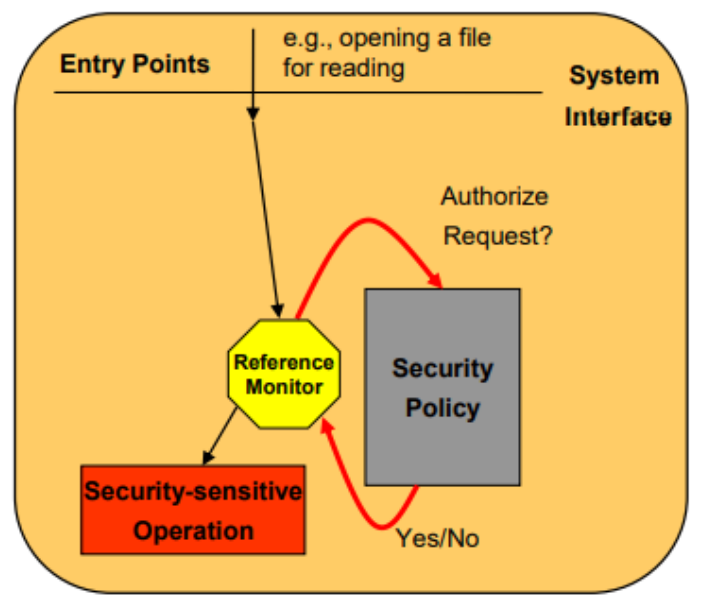
\includegraphics[width=\linewidth]{reference_monitor.png}

    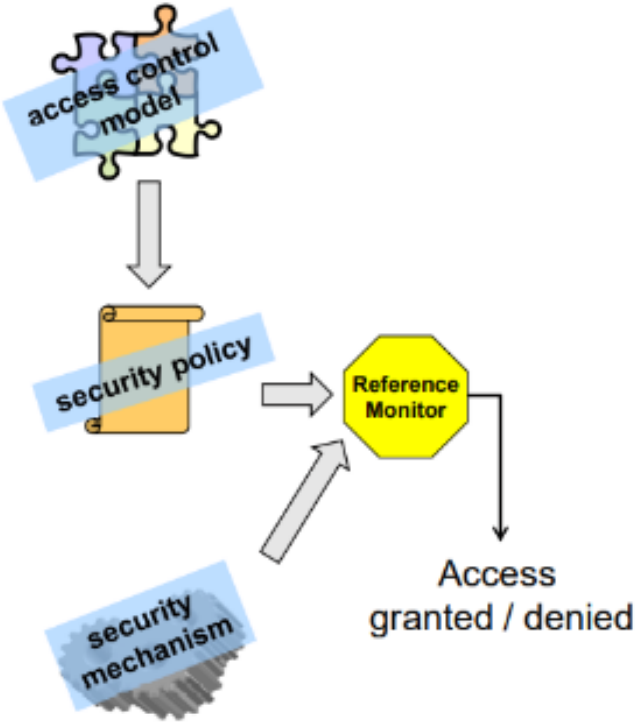
\includegraphics[width=\linewidth]{reference_monitor2.png}
\end{concept}

\begin{definition}{Security Policy}\\
    \begin{itemize}
        \item Defines who is allowed to do what on a system
        \item Should be flexible in terms of configuration
    \end{itemize}
\end{definition}

\begin{definition}{Security Mechanism}\\
    \begin{itemize}
        \item Method / Structure used to implement the security policy
    \end{itemize}
\end{definition}

\subsection{Multi-tier Applications}

\begin{concept}{Multi-tier Applications}\\
    \begin{itemize}
        \item Based on Multi-Tier architecture
        \item Three-tier architecture:
        \begin{itemize}
            \item Presentation
            \item Logic  
            \item Data
        \end{itemize}
    \end{itemize}
\end{concept}

\subsubsection{Impersonation / Delegation}

\begin{definition}{Impersonation / Delegation}\\
    \begin{itemize}
        \item The subject "survives" beyond the middle tier
        \item Generate impersonation token that reflects the subject's access control data
    \end{itemize}
    
    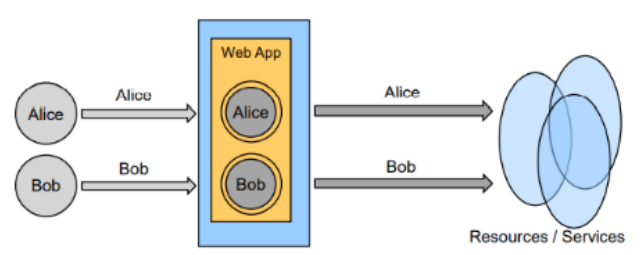
\includegraphics[width=\linewidth]{impersonation_diagram.png}
\end{definition}

\subsubsection{Trusted Application Model}

\begin{definition}{Trusted Application Model}\\
    \begin{itemize}
        \item Access to backend via service account
        \item Requests are granted/denied to subjects based on a set of access policies
    \end{itemize}
    
    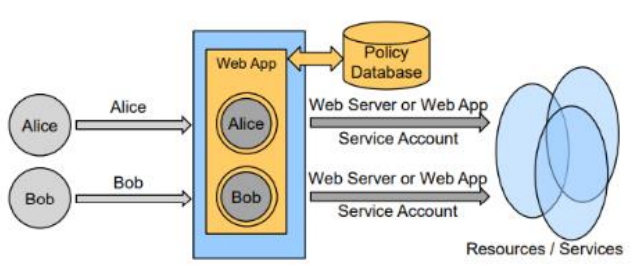
\includegraphics[width=\linewidth]{application_model.png}
\end{definition}

\subsection{Access Control Models}

\begin{concept}{Access Control Models}\\
    Access control models are framework dictating how subjects access objects.
\end{concept}

\subsubsection{Discretionary Access Control (DAC)}

\begin{definition}{Discretionary Access Control (DAC)}\\
    \begin{itemize}
        \item Based on discretion of the owner of an object
        \item Example: Modern OS (Windows, Linux, Mac)
        \item Usually includes a user that can bypass restrictions (root / admin)
        \item Uses Access Control List ACL or Capabilities
    \end{itemize}
    
    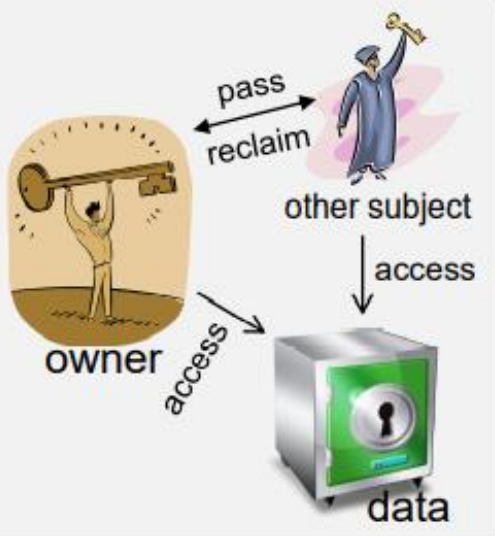
\includegraphics[width=0.3\linewidth]{DAC_diag.png}
\end{definition}

\subsubsection{Mandatory Access Control (MAC)}

\begin{definition}{Mandatory Access Control (MAC)}\\
    \begin{itemize}
        \item A system wide policy determines who is allowed to access
        \item Individual user cannot alter
        \item Policy is configured by a policy administrator
    \end{itemize}
    
    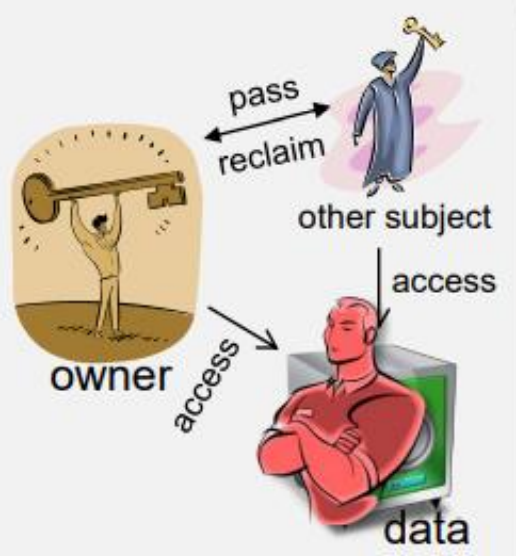
\includegraphics[width=0.3\linewidth]{MAC_diag.png}
\end{definition}

\begin{concept}{Bell-LaPadula Model}\\
    \begin{itemize}
        \item Multi-level security model
        \item Directed towards confidentiality
        \item No read up
        \item No write down
    \end{itemize}
\end{concept}

\begin{concept}{Biba Model}\\
    \begin{itemize}
        \item Directed towards integrity
        \item No write up
        \item No read down
    \end{itemize}
\end{concept}

\subsubsection{Role-Based Access Control (RBAC)}

\begin{definition}{Role-Based Access Control (RBAC)}\\
    \begin{itemize}
        \item Decision based on the users' role within an organization
        \item Example: Oracle DBMS
        \item A role defines a set of transactions allowed for its members
        \item Not provided by OS
        \item Principle of least privilege
    \end{itemize}
    
    
\end{definition}

\begin{concept}{RBAC Components}\\
    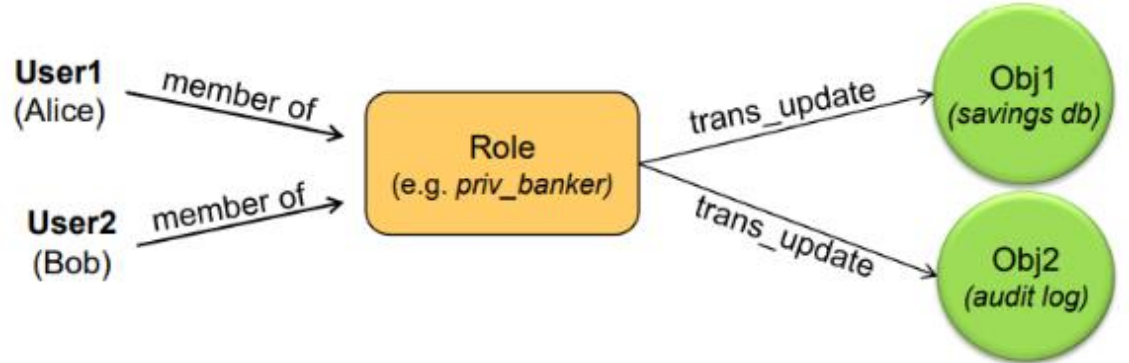
\includegraphics[width=\linewidth]{RBAC.png}
\end{concept}

\subsection{Access Control Model Comparison}

\begin{theorem}{Access Control Models Summary}\\
    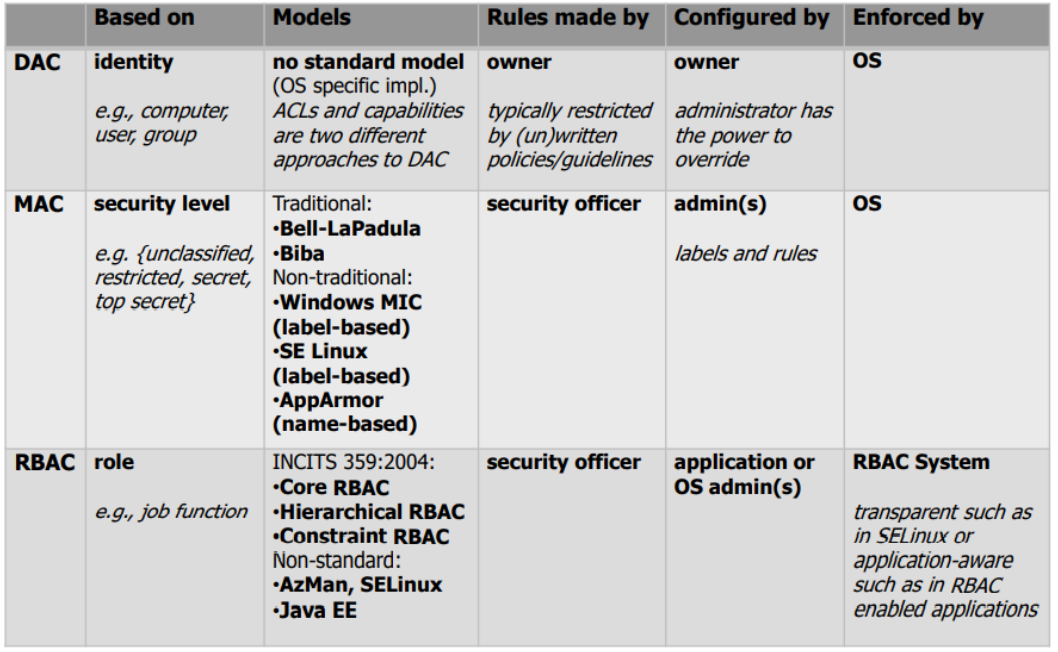
\includegraphics[width=\linewidth]{ACM_overview.png}
    % Based on | Models | Rules made by | Configured by | Enforced by
    
    \textbf{DAC (Discretionary Access Control):}
    \begin{itemize}
        \item Based on: Identity (e.g., computer, user, group)
        \item Models: No standard model (OS specific impl.), ACLs and capabilities
        \item Rules made by: Owner, typically restricted by policies/guidelines
        \item Configured by: Owner, administrator has power to override
        \item Enforced by: OS
    \end{itemize}
    
    \textbf{MAC (Mandatory Access Control):}
    \begin{itemize}
        \item Based on: Security level (e.g., unclassified, restricted, secret, top secret)
        \item Models: Windows MIC (label-based), SE Linux (label-based), AppArmor (name-based)
        \item Rules made by: Security officer
        \item Configured by: Admin(s), labels and rules
        \item Enforced by: OS
    \end{itemize}
    
    \textbf{RBAC (Role-Based Access Control):}
    \begin{itemize}
        \item Based on: Role (e.g., job function)
        \item Models: INCITS 359:2004 (Core RBAC, Hierarchical RBAC, Constraint RBAC), Non-standard (SELinux, Java EE)
        \item Rules made by: Business/security officer
        \item Configured by: Application or OS admin(s)
        \item Enforced by: RBAC System (transparent such as in SELinux or application-aware)
    \end{itemize}
\end{theorem}